%%%%%%%%%%%%%%%%%%%%%%%%%%%%%%%%%%%%%%%%%%%%%%%%%%%%%%%%%%%%%%%%%
% MUW Presentation
% LaTeX Template
% Version 1.0 (27/12/2016)
%
% License:
% CC BY-NC-SA 4.0 (http://creativecommons.org/licenses/by-nc-sa/3.0/)
%
% Created by:
% Nicolas Ballarini, CeMSIIS, Medical University of Vienna
% nicoballarini@gmail.com
% http://statistics.msi.meduniwien.ac.at/
%
% Customized for UAH by:
% David F. Barrero, Departamento de Automática, UAH
%%%%%%%%%%%%%%%%%%%%%%%%%%%%%%%%%%%%%%%%%%%%%%%%%%%%%%%%%%%%%%%%%

\documentclass[10pt,compress]{beamer} % Change 10pt to make fonts of a different size
\mode<presentation>

\usepackage[spanish]{babel}
\usepackage{fontspec}
\usepackage{tikz}
\usepackage{etoolbox}
\usepackage{xcolor}
\usepackage{xstring}
\usepackage{listings}
\usepackage{multicol}
\usepackage{tabularx}
\usepackage{tikz}
\usetikzlibrary{matrix,chains,positioning,decorations.pathreplacing,arrows,shapes}

\usetheme{UAH}
\usecolortheme{UAH}
\setbeamertemplate{navigation symbols}{} 
\setbeamertemplate{caption}[numbered]

%%%%%%%%%%%%%%%%%%%%%%%%%%%%%%%%%%%%%%%%%%%%%%%%%%%%%%%%%%%%%%%%%
%% Presentation Info
\title[Scientific programming crash course]{Scientific Programming in Python crash course}
\author{\asignatura\\\carrera}
\institute{}
\date{Departamento de Automática}
%%%%%%%%%%%%%%%%%%%%%%%%%%%%%%%%%%%%%%%%%%%%%%%%%%%%%%%%%%%%%%%%%


%%%%%%%%%%%%%%%%%%%%%%%%%%%%%%%%%%%%%%%%%%%%%%%%%%%%%%%%%%%%%%%%%
%% Descomentar para habilitar barra de navegación superior
\setNavigation
%%%%%%%%%%%%%%%%%%%%%%%%%%%%%%%%%%%%%%%%%%%%%%%%%%%%%%%%%%%%%%%%%

%%%%%%%%%%%%%%%%%%%%%%%%%%%%%%%%%%%%%%%%%%%%%%%%%%%%%%%%%%%%%%%%%
%% Configuración de logotipos en portada
%% Opacidad de los logotipos
\newcommand{\opacidad}{1}
%% Descomentar para habilitar logotipo en pié de página de portada
\renewcommand{\logoUno}{Images/isg.png}
%% Descomentar para habilitar logotipo en pié de página de portada
%\renewcommand{\logoDos}{Images/CCLogo.png}
%% Descomentar para habilitar logotipo en pié de página de portada
%\renewcommand{\logoTres}{Images/ALogo.png}
%% Descomentar para habilitar logotipo en pié de página de portada
%\renewcommand{\logoCuatro}{Images/ELogo.png}
%%%%%%%%%%%%%%%%%%%%%%%%%%%%%%%%%%%%%%%%%%%%%%%%%%%%%%%%%%%%%%%%%

%%%%%%%%%%%%%%%%%%%%%%%%%%%%%%%%%%%%%%%%%%%%%%%%%%%%%%%%%%%%%%%%%
%% FOOTLINE
%% Comment/Uncomment the following blocks to modify the footline
%% content in the body slides. 


%% Option A: Title and institute
\footlineA
%% Option B: Author and institute
%\footlineB
%% Option C: Title, Author and institute
%\footlineC
%%%%%%%%%%%%%%%%%%%%%%%%%%%%%%%%%%%%%%%%%%%%%%%%%%%%%%%%%%%%%%%%%

\begin{document}

%%%%%%%%%%%%%%%%%%%%%%%%%%%%%%%%%%%%%%%%%%%%%%%%%%%%%%%%%%%%%%%%%
% Use this block for a blue title slide with modified footline
{\titlepageBlue
    \begin{frame}
        \titlepage
    \end{frame}
}

\institute{\asignatura}

\begin{frame}[plain]{}
	\begin{block}{Objectives}
		\begin{enumerate}
		\item Introduce scientific programming problems
		\item Efficient matrix computations in Python
		\item Visualize data in Python
		\end{enumerate}
	\end{block}

   \begin{block}{Bibliography}
       Jake VanderPlas. \textit{Python Data Science Handbook}. Chapter 1. O'Reilly. \href{https://jakevdp.github.io/PythonDataScienceHandbook/}{(Link)}.
   \end{block}

\end{frame}

{
\disableNavigation{white}
\begin{frame}[shrink]{Table of Contents}
 \frametitle{Table of Contents}
 \begin{multicols}{2}
 \tableofcontents
 \end{multicols}
  % You might wish to add the option [pausesections]
\end{frame}
}

\section{The data scientist toolkit}

\subsection{Motivation}

\begin{frame}{The data scientist toolkit}{Motivation}
	Data science is about manipulating data
	\begin{itemize}
		\item Need of specialized tools
		\item Two main languajes: R and Python
	\end{itemize}
	Python is a general purpose programming language
	\begin{itemize}
		\item Easy integration 
		\item Huge ecosystem of packages and tools
	\end{itemize}
	Need of data-oriented tools
	\begin{itemize}
		\item Features provided by third-party tools
	\end{itemize}
\end{frame}

\subsection{Overview}

\begin{frame}{The data scientist toolkit}{Overview}
   \begin{tabular}{cll}\hline
       \textbf{Tool}& \textbf{Type} & \textbf{Description}\\ \hline
	   \texttt{conda} 	& Software & Python environments and package management \\
	   \texttt{iPython} & Software & Advaced Python interpreter \\
	   \texttt{Jupiter} & Software & Python notebooks (Python interpreter) \\
	   \texttt{Numpy}   & Package  & Efficient array operations \\
	   \texttt{Pandas}  & Package  & Dataframe support \\
	   \texttt{Matplotlib} & Package & Data visualization \\
	   \texttt{Seaborn} & Package & Data visualization with dataframes \\
	   \texttt{Scikit-learn} & Package & AI/ML package for Python \\
	   \hline
   \end{tabular}
\end{frame}

\subsection{Anaconda}
\begin{frame}{The data scientist toolkit}{Anaconda}
    \begin{columns}
 	   \column{.6\textwidth}
   Most of those tools are packaged in \textit{Anaconda}
   \begin{itemize}
   		\item Python distribution for Data Science
		\item Environment management for Python
		\item Package management system
	\end{itemize}

	Anaconda provides \texttt{conda}
	\begin{itemize}
		\item Packages management tool
		\item Environment management for Python
	\end{itemize}

	In addition, Anaconda provides \texttt{Spyder}
	\begin{itemize}
		\item Python IDE designed for Data Science
	\end{itemize}

 		\column{.4\textwidth}
		
\includegraphics[width=0.6\textwidth]{figs/Anaconda_Logo.png} \\\bigskip
		
\includegraphics[width=0.5\textwidth]{figs/spyder.png}	
		%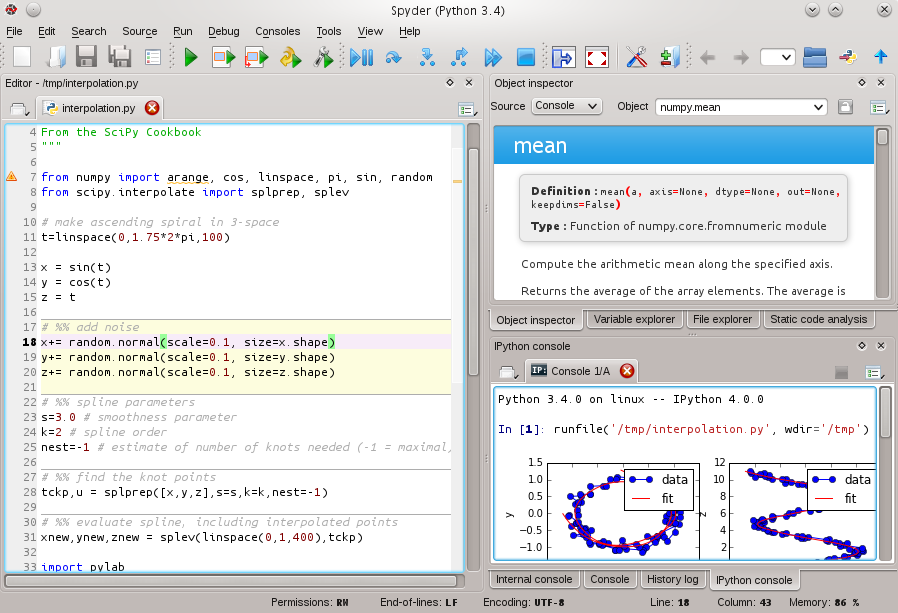
\includegraphics[width=0.6\textwidth]{figs/spyder-ide.png}	
	\end{columns}
\end{frame}

\subsection{Conda}
\begin{frame}{The data scientist toolkit}{Conda crush introduction}
    \begin{columns}
 	   \column{.5\textwidth}
	   \begin{block}{Conda environment for Data Science}
	   	\begin{enumerate}
			\item \texttt{conda create --name ml seaborn=0.9.0}
			\item \texttt{source activate ml}
			\item \texttt{conda install ipython}
			\item \texttt{conda install nb\_conda}
			\item \texttt{conda install scikit-learn}
		\end{enumerate}
	   \end{block}

 		\column{.5\textwidth}
		List environments: \\ \quad \texttt{conda info --envs}\\
		Activate environment: \\ \quad \texttt{source activate <env>}\\
		Install package: \\ \quad \texttt{conda install <package>}\\
		List packages: \\ \quad \texttt{conda list}\\
		Exit environment (Linux): \\ \quad \indent \texttt{deactivate}
	\end{columns}
\end{frame}

\section{numpy}

\subsection{Understanding Data Types in Python}

\begin{frame}{Introduction}{Understanding Data Types in Python (I)}
    %Python supports matrices by default
    %\begin{itemize}
    %    \item Why do we need additional support?
	%\end{itemize}

    \begin{columns}
 	   \column{0.5\textwidth}
			
			\begin{block}{\footnotesize{Static typing}}
			\vspace{-0.2cm} 
				\lstinputlisting[basicstyle=\ttfamily\scriptsize,language=C]{code/static.c}
			\vspace{-0.2cm} 
			\end{block}

			\begin{itemize}
				\item Data types must be declared
				\item Data types cannot change
				\item Error detection in compilation
				\item Variables names are, basicly, labels
			\end{itemize}
			
 	   \column{0.5\textwidth}
			\begin{block}{\footnotesize{Dynamic typing}}
			\vspace{-0.2cm} 
				\lstinputlisting[basicstyle=\ttfamily\scriptsize]{code/dynamic.py}
			\vspace{-0.2cm} 
			\end{block}

			\begin{itemize}
				\item Data types are not declared
				\item Data types can change
				\item Error detection in run-time
				\item Variables are complex data structures (even for simple types)
			\end{itemize}
	\end{columns}
\end{frame}

\begin{frame}{Introduction}{Understanding Data Types in Python (II)}
    %Python supports matrices by default
    %\begin{itemize}
    %    \item Why do we need additional support?
	%\end{itemize}

	Dynamic typing must be implemented somewhere ...

    \begin{columns}
 	   \column{0.5\textwidth}
			\begin{block}{\footnotesize{Python 3.4 source code}}
			\vspace{-0.2cm} 
				\lstinputlisting[basicstyle=\ttfamily\scriptsize, language=C]{code/long.c}
			\vspace{-0.2cm} 
			\end{block}

 	   \column{0.5\textwidth}
			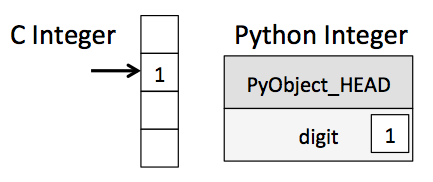
\includegraphics[width=\textwidth]{figs/cint_vs_pyint.png}	
	\end{columns}

\end{frame}

\begin{frame}[fragile]{Introduction}{Understanding Data Types in Python (III)}
	\begin{columns}
 	   \column{0.5\textwidth}
			A Python list may contain different types

 	   \column{0.5\textwidth}
	   \begin{exampleblock}{}
			\vspace{-0.2cm} 
			\lstinputlisting[basicstyle=\ttfamily\scriptsize]{code/lists.txt}
			\vspace{-0.2cm} 
		\end{exampleblock}
	\end{columns}

	\bigskip

	\centering 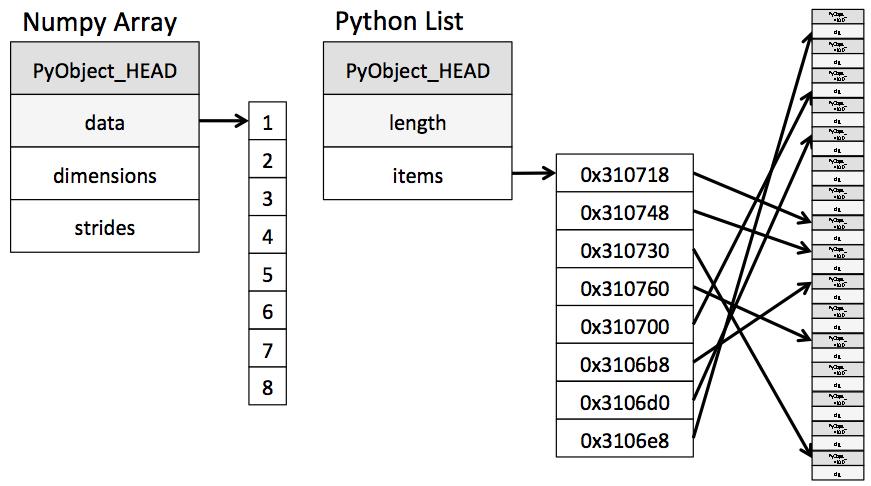
\includegraphics[width=0.8\textwidth]{figs/array_vs_list.png}	
\end{frame}

\begin{frame}[fragile]{Introduction}{Understanding Data Types in Python (IV)}
	Standard Python data types are powerful and flexible
	\begin{itemize}
		\item Flexibility has a price: Reduced performance
		\item Not an big issue in generic programming
		\item A big issue in scientific programming
		\item We require efficient data manipulation mechanisms: NumPy
	\end{itemize}
	NumPy: Python package for numeric computation
	\begin{itemize}
		\item Efficient array implementation
		\item Fast mathematical functions
		\item Random numbers generation
		\item Static data types: Less flexibility
	\end{itemize}
	Most Python modules for AI/ML depend on NumPy, in particular
	\begin{itemize}
		\item Pandas (dataframes), Scikit-learn (ML), Seaborn (data visualization)
	\end{itemize}
\end{frame}

\section{NumPy}
\subsection{Introduction}

\begin{frame}[fragile]{NumPy}{Introduction}
	\begin{columns}
 	   \column{0.6\textwidth}
		NumPy must be imported in order to be available
		\begin{itemize}
			%\item By convention, \texttt{import numpy as np}
			\item You can use \texttt{np?} or \texttt{np.<TAB>}
		\end{itemize}

		The main component of NumPy is \alert{ndarray}
		\begin{itemize}
			\item Python object
			\item Efficient matrix representation
			\item Homogeneus elements
		\end{itemize}

 	   \column{0.4\textwidth}
		\begin{block}{\footnotesize{Convention}}
		\vspace{-0.2cm} 
\begin{lstlisting}
import numpy as np
\end{lstlisting}
		\vspace{-0.2cm} 
		\end{block}

		\begin{exampleblock}{}
		\vspace{-0.2cm} 
\begin{lstlisting}
In [1]: array = np.array([1,2,3])
In [2]: array
Out[1]: array([1, 2, 3])
In [3]: array = np.array([[1,2],[3,4]])
\end{lstlisting}
		\vspace{-0.2cm} 
		\end{exampleblock}
	\end{columns}
\end{frame}

\subsection{NumPy array attributes}
\begin{frame}[fragile]{NumPy}{NumPy array attributes}
	\begin{columns}
 	   \column{0.5\textwidth}
		Ndarray objects expose several attributes
		\begin{itemize}
			\item \texttt{ndim}: Dimensions
			\item \texttt{shape}: Size of each dimension
			\item \texttt{size}: Number of elements
			\item \texttt{dtype}: Data type
			\item \texttt{itemsize}: Size of each element (in bytes)
			\item \texttt{nbytes}: Size of the array (in bytes)
		\end{itemize}

 	   \column{0.5\textwidth}
		\begin{exampleblock}{}
		\vspace{-0.2cm} 
			\begin{lstlisting}
x = np.random.randint(10, size=(3, 4))
print("x ndim: ", x.ndim)
print("x shape:", x.shape)
print("x size: ", x.size)
print("dtype:", x.dtype)
print("itemsize:", x.itemsize)
print("nbytes:", x.nbytes)
\end{lstlisting}
		\vspace{-0.2cm} 
		\end{exampleblock}
	\end{columns}
\end{frame}

\subsection{NumPy data types}
\begin{frame}[fragile]{NumPy}{NumPy data types}
	\begin{columns}
 	   \column{0.4\textwidth}
	   Python is implemented in C
	   \begin{itemize}
	   	\item Data types in NumPy are based on those in C
	   \end{itemize}
	   Two styles to declare types
	   \begin{itemize}
	   	\item String:\\ \texttt{np.zeros(10, dtype='int16')}
		\item NumPy object: \texttt{np.zeros(10, dtype=np.int16)}
	   \end{itemize}

 	   \column{0.6\textwidth}
	\footnotesize{
    \begin{tabular}{ll}\hline
       \textsc{Data type} &  \textsc{Description}\\ \hline
	   \texttt{bool\_} & Boolean (True or False) stored as a byte  \\
	   \texttt{int\_} & Default integer type  \\
	   \texttt{intc} & Identical to C  \\
	   \texttt{intp} & Integer used for indexing  \\
	   \texttt{int8} & Byte  \\
	   \texttt{int16} & Integer  \\
	   \texttt{int32} & Integer  \\
	   \texttt{int64} & Integer  \\
	   \texttt{uint8} & Unsigned integer  \\
	   \texttt{uint16} & Unsigned integer  \\
	   \texttt{uint32} & Unsigned integer  \\
	   \texttt{uint64} & Unsigned integer  \\
	   \texttt{float\_} & Shorthand for float64  \\
	   \texttt{float16} & Half precision float  \\
	   \texttt{float32} & Single precision float  \\
	   \texttt{float64} & Double precision float  \\
	   \texttt{complex\_} & Shorthand for complex128  \\
	   \texttt{complex64} & Complex number  \\
	   \texttt{complex128} & Complex number  \\\hline
    \end{tabular}
	}
	\end{columns}
\end{frame}

\subsection{NumPy notebook}
\begin{frame}{NumPy}{NumPy notebook}
    \begin{columns}
 	   \column{0.5\textwidth}
			\begin{block}{NumPy notebook}
			\href{https://github.com/dfbarrero/dataCourse/blob/master/numpy/numpy.ipynb}{(Link to notebook)}
			\end{block}
	\end{columns}
\end{frame}

\section{Pandas}
\subsection{Introduction}

\begin{frame}[fragile]{Pandas}{Introduction}
	\begin{columns}
 	   \column{0.6\textwidth}
		A DS/ML workflow needs more features
		\begin{itemize}
			\item Missing data
			\item Data input
			\item Operations on groups
			\item Label columns and rows
		\end{itemize}
		Pandas provides all those features, and more
		\begin{itemize}
			\item Pandas = \textbf{PAN}el \textbf{DA}ta \textbf{S}ystem
			\item Built on NumPy's ndarray
			\item Provides \alert{dataframes}
		\end{itemize}
		Pandas provides two main objects
		\begin{itemize}
			\item \texttt{Series} and \texttt{DataFrame}
		\end{itemize}

 	   \column{0.4\textwidth}
		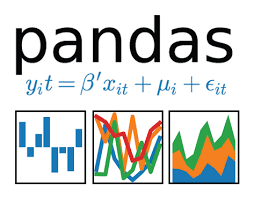
\includegraphics[width=\textwidth]{figs/pandas.png}	

		\begin{block}{\footnotesize{Convention}}
		\vspace{-0.2cm} 
			\begin{lstlisting}
import numpy as np
import pandas as pd
\end{lstlisting}
\vspace{-0.2cm} 
\end{block}

	\end{columns}
\end{frame}

\subsection{The Pandas \texttt{Series} object}

\begin{frame}[fragile]{Pandas}{The Pandas \texttt{Series} object (I)}
	\begin{columns}
 	   \column{0.6\textwidth}

		A \texttt{Series} is a one-dimensional array of indexed data
		\begin{itemize}
			\item NumPy arrays indices are implicit (i.e. its position)
			\item Series indices are explicit, and can be any type
		\end{itemize}
		Two attributes
		\begin{itemize}
			\item \texttt{values}: ndarray
			\item \texttt{index}: \texttt{pd.Index} object
		\end{itemize}
		Two indices
		\begin{itemize}
			\item Implicit: Regular index
			\item Explicit: Custom index
		\end{itemize}

 	   \column{0.4\textwidth}
	   \centering
      	\begin{tabularx}{2.7cm}{|c|c|}
			\hline
       		\textsc{Index} &  \textsc{Values}\\ \hline
       		\textit{'a'} & 0.25 \\
       		\textit{'b'} & 0.5  \\
       		\textit{'c'} & 0.75 \\
       		\textit{'d'} & 0.99 \\\hline
    	\end{tabularx}

		\bigskip

		\begin{exampleblock}{}
		\vspace{-0.2cm} 
			\begin{lstlisting}
data = pd.Series([0.25, 0.5, 0.75, 1.0])
data.values
data.index
data[1:3]
\end{lstlisting}
		\vspace{-0.2cm} 
		\end{exampleblock}
	\end{columns}
\end{frame}

\begin{frame}[fragile]{Pandas}{The Pandas \texttt{Series} object (II)}
	\begin{columns}
 	   \column{0.8\textwidth}
		\begin{exampleblock}{\footnotesize{Custom indices}}
		\vspace{-0.2cm} 
			\begin{lstlisting}
In[1] : data = pd.Series([0.25, 0.5, 0.75, 1.0],
    index=['a', 'b', 'c', 'd'])
In [2]: data
Out[1]: 
    a    0.25
    b    0.50
    c    0.75
    d    1.00
    dtype: float64

    In [3]: data['a']
    Out[2]: 0.25
    In [4]: data[0]
    Out[3]: 0.25
\end{lstlisting}
\vspace{-0.2cm} 
\end{exampleblock}
	\end{columns}
\end{frame}

\subsection{The Pandas \texttt{DataFrame} object}

\begin{frame}{Pandas}{The Pandas \texttt{DataFrame} object (I)}
	\begin{columns}
 	   \column{0.6\textwidth}
		A \texttt{DataFrame} is a 2-D tabular data structure
		\begin{itemize}
			\item Similar to a spreadsheet
			\item Homogeneous columns
			\item Heterogeneous rows
		\end{itemize}
		Two read-only attributes, both \texttt{pd.Index}
		\begin{itemize}
			\item \texttt{index}: Rows
			\item \texttt{columns}: Columns
		\end{itemize}

 	   \column{0.4\textwidth}
		\centering 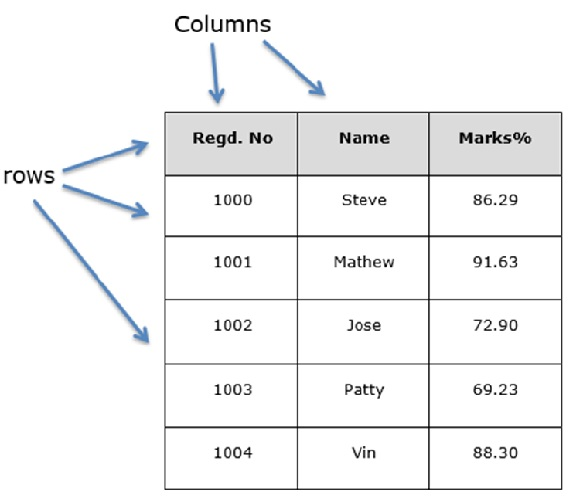
\includegraphics[width=\textwidth]{figs/structure_table.jpg}\\
		\tiny \href{https://www.tutorialspoint.com/python\_pandas/python\_pandas\_dataframe.htm}{(Source)}
	\end{columns}
\end{frame}

\begin{frame}[fragile]{Pandas}{The Pandas \texttt{DataFrame} object (II)}
	\begin{columns}
	   \column{\textwidth}
		\begin{exampleblock}{\footnotesize{DataFrame example}}
		\vspace{-0.2cm} 
			\begin{lstlisting}
In [1]:  import seaborn as sns

In [2]:  iris = sns.load_dataset('iris')
In [3]:  iris.head()

Out[1]:
sepal_length  sepal_width  petal_length  petal_width species
0           5.1          3.5           1.4          0.2  setosa
1           4.9          3.0           1.4          0.2  setosa
2           4.7          3.2           1.3          0.2  setosa
3           4.6          3.1           1.5          0.2  setosa
4           5.0          3.6           1.4          0.2  setosa
In [246]: iris.columns
Out[246]: 
Index(['sepal_length', 'sepal_width', 'petal_length', 
        'petal_width', 'species'], dtype='object')
\end{lstlisting}
\vspace{-0.2cm} 
		\end{exampleblock}
	\end{columns}
\end{frame}

\begin{frame}[fragile]{Pandas}{The Pandas \texttt{DataFrame} object (III)}
	Read from a file
	\begin{itemize}
		\item Excel:\\
		\texttt{pd.read\_excel('filename.xlsx', sheetname='mysheet')}
		\item CSV (very common!!!): \texttt{pd.read\_csv('filename.csv')}
	\end{itemize}

	\begin{exampleblock}{CSV example}
		\begin{lstlisting}
# This CSV file contains data about weights and heights
"id", "weight","height","sex",  "race"
1,    143.5,   81.6,    "Female","White"
2,    109.1,   83.7,    "Female","Black"
4,    104.8,   54.6,    "Female","Hisp"
7,    130.2,   81.7,    "Male",  "White"
\end{lstlisting}
	\end{exampleblock}
	CVS can be exported from MS Excel or programatically
\end{frame}

\subsection{Pandas notebook}
\begin{frame}{Pandas}{Pandas notebook}
    \begin{columns}
 	   \column{0.5\textwidth}
			\begin{block}{NumPy notebook}
			\href{https://github.com/dfbarrero/dataCourse/blob/master/pandas/Pandas.ipynb}{(Link to notebook)}
			\end{block}
	\end{columns}
\end{frame}

\section{Data visualization}
\subsection{Introduction}

\begin{frame}[plain]{Datavisualization}{Motivation (I)}
	\centering 
\includegraphics[width=0.8\textwidth]{figs/chart-selection-diagram.png}\\
	\centering \tiny \href{https://flex.bi/create-beautiful-dashboard-works/}{(Source)}\\
	\href{http://experception.net/Franconeri_ExperCeptionDotNet_ChartChooser.pdf}{(Alternative resource)}
\end{frame}


\subsection{Matplotlib}

\begin{frame}[fragile]{Data visualization}{Matplotlib (I)}
	\begin{columns}
    \column{0.5\textwidth}
	Matplotlib is a Python package
	\begin{itemize}
		\item Based on NumPy
		\item Imitates Matlab
	\end{itemize}
	Three operation modes
	\begin{itemize}
		\item Scripts. \\Must use \texttt{plt.show()} to enter event loop. Use it once!
		\item IPython shell. \\Must use \texttt{\%matplotlib}
		\item IPython notebook. Two modes
		\begin{itemize}
			\item \texttt{\%matplotlib inline}
			\item \texttt{\%matplotlib notebook}
		\end{itemize}
	\end{itemize}

    \column{0.5\textwidth}
	\begin{block}{\footnotesize{Convention}}
	\vspace{-0.2cm} 
	\begin{lstlisting}
import matplotlib as mpl
import matplotlib.pyplot as plt
\end{lstlisting}
	\vspace{-0.2cm} 
	\end{block}

	\begin{exampleblock}{\footnotesize{myplot.py}}
	\vspace{-0.2cm} 
	\begin{lstlisting}
import matplotlib.pyplot as plt
import numpy as np

x = np.linspace(0, 10, 100)

plt.plot(x, np.sin(x))
plt.plot(x, np.cos(x))

plt.show()
\end{lstlisting}
	\vspace{-0.2cm} 
	\end{exampleblock}

	\end{columns}
\end{frame}

\begin{frame}[fragile]{Data visualization}{Matplotlib (II)}
	Matplotlib comes with two interfaces
	\begin{itemize}
		\item Matlab-like. Old-fashioned function-oriented API.
		\item Object-oriented. Object-oriented and more powerfull API.
	\end{itemize}

	\begin{columns}
    \column{0.5\textwidth}
	\begin{exampleblock}{Matlab API}
	\vspace{-0.2cm} 
	\begin{lstlisting}
	plt.figure()  # create a plot

	# create the first of two panels and set current axis
	plt.subplot(2, 1, 1) # (rows, columns, panel number)
	plt.plot(x, np.sin(x))

	# create the second panel and set current axis
	plt.subplot(2, 1, 2)
	plt.plot(x, np.cos(x));
	\end{lstlisting}
	\vspace{-0.2cm} 
	\end{exampleblock}

    \column{0.5\textwidth}
	\begin{exampleblock}{OO API}
	\vspace{-0.2cm} 
	\begin{lstlisting}
	plt.figure()  # create a plot

	# create the first of two panels and set current axis
	plt.subplot(2, 1, 1) # (rows, columns, panel number)
	plt.plot(x, np.sin(x))

	# create the second panel and set current axis
	plt.subplot(2, 1, 2)
	plt.plot(x, np.cos(x));
	\end{lstlisting}
	\vspace{-0.2cm} 
	\end{exampleblock}
	\end{columns}
\end{frame}

\subsection{Matplotlib notebook}
\begin{frame}{Pandas}{Matplotlib notebook}
    \begin{columns}
 	   \column{0.5\textwidth}
			\begin{block}{Matplotlib notebook}
			\href{https://github.com/dfbarrero/dataCourse/blob/master/dataviz/DatavizWithMatplotlib.ipynb}{(Link to notebook)}
			\end{block}
	\end{columns}
\end{frame}

\subsection{Searborn}

\begin{frame}[fragile]{Data visualization}{Seaborn (I)}
	\begin{columns}
    \column{0.65\textwidth}
	Seaborn is a modern data-visualization Python package
	\begin{itemize}
		\item Based on matplotlib
		\item ... it uses matplotlib indeed
		\item Pandas-aware
		\item High level
		\item Advanced visualizations
		\item Easy to use
	\end{itemize}
	Still under development! (v. 0.9)
    \column{0.35\textwidth}
	\begin{block}{\footnotesize{Convention}}
	\vspace{-0.2cm} 
	\begin{lstlisting}
import seaborn as sns
\end{lstlisting}
	\vspace{-0.2cm} 
	\end{block}

	\begin{alertblock}{}
	\vspace{-0.2cm} 
	\footnotesize{This documentation is for Seaborn 0.9 or newer}
	\vspace{-0.2cm} 
	\end{alertblock}

	\end{columns}
\end{frame}

\begin{frame}[fragile]{Data visualization}{Seaborn (II)}
	\begin{columns}
    \column{0.5\textwidth}
	Display initialization
	\begin{itemize}
		\item \texttt{plt.show()}
		\item \texttt{\%matplotlib}
	\end{itemize}
	Style initialization
	\begin{itemize}
		\item Default Seaborn style \texttt{sns.set()}
		\item By default, same style than matplotlib
	\end{itemize}
	Several functions ...
	\begin{itemize}
		\item ... similar parameters
	\end{itemize}

    \column{0.5\textwidth}
	\begin{block}{Parameters}
	\begin{itemize}
		\item x: Data axis x
		\item y: Data axis Y
		\item data: Dataframe name
		\item hue: Color
		\item style: Style
		\item sizes: Size
		\item kind: Alternate representation
	\end{itemize}
	\end{block}
	\end{columns}
\end{frame}

\begin{frame}[fragile]{Data visualization}{Seaborn (III)}
	\begin{columns}
    \column{0.4\textwidth}
		\begin{block}{Typical Seaborn usage}
		\begin{enumerate}
			\item Prepare data
			\item Set up aesthetics
			\item Plot
			\item Customize the plot
		\end{enumerate}
	\end{block}

    \column{0.6\textwidth}
		\begin{exampleblock}{}
			\vspace{-0.2cm} 
			\begin{lstlisting}[basicstyle=\tiny]
import matplotlib.pyplot as plt
import seaborn as sns
# Prepare data
tips = sns.load_dataset("tips")
# Set up aesthetics
sns.set_style("whitegrid")
# Plot
g = sns.lmplot(x="tip",y="total_bill", data=tips,aspect=2)
# Plot customization
g = (g.set_axis_labels("Tip","Total bill(USD)").set(xlim=(0,10),ylim=(0,100)))
plt.title("title")
plt.show(g)
\end{lstlisting}
		\vspace{-0.2cm} 
		\end{exampleblock}

		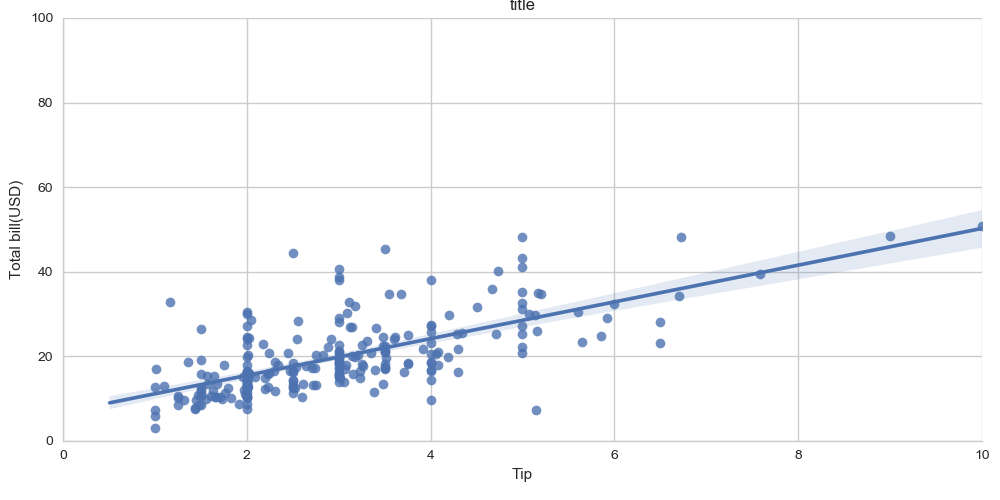
\includegraphics[width=\textwidth]{figs/sns-lm.png}\\
	\end{columns}
\end{frame}

\subsection{Seaborn notebook}
\begin{frame}{Seaborn}{Seaborn notebook}
    \begin{columns}
 	   \column{0.5\textwidth}
			\begin{block}{Seaborn notebook}
			\href{https://github.com/dfbarrero/dataCourse/blob/master/dataviz/DatavizWithSeaborn.ipynb}{(Link to notebook)}
			\end{block}
	\end{columns}
\end{frame}


\end{document}
